
%|  Name  | TODO | ONGOING | DONE |
%|--------|------|---------|------|
%| Dana   | x    |         |      |
%| Gerd   |      |         | x    |
%| Glenn  |      |         |  x   |
%| Jordan | x    |         |      |
%| Luke   | x    |         |      |
%| Matt   |      |         | x    |
%| Neil   | x    |         |      |
%| Scot   | x    |         | x     |


%CLEANUP \todo[inline]{Owner: Gerd -- Priority: High -- Effort: S -- Completion: 100\%}

Throughout this tour, we describe the run-time use of the term `HDF5 library', which provides complete coverage of the architectural concepts in different contexts with different meanings. It should be clear from the context which meaning is intended, but we list them here for completeness. The term `HDF5 library' refers to one of the following:

\begin{enumerate}
    \item An architectural concept.
    \item A body of source code, versions of which can be found on GitHub~\cite{libhdf52023}.
    \item A binary compiled and configured for a particular platform using CMake~\cite{cmake2023} or Autotools~\cite{autotools2023}.
    \item An HDF5 library binary loaded into the context of a process, a library \textit{instance}.
    \item The internal state of an HDF5 library instance.
    \item A combination of one or more of the above, in a generic sense.
\end{enumerate}

We begin with a 35,000-foot overview of how the HDF5 library is structured. As shown in Figure~\ref{fig:vol-arch}, \textit{the primary purpose of the HDF5 library is to provide mappings between in-memory representations of HDF5 objects or entities and storage representations}. There are many possible implementations of such mappings, all of which share the HDF5 data model and library API. The API comprises two types of functions: functions dealing with the management of virtual objects and functions configuring API behavior or virtual object support functions. In Figure~\ref{fig:vol-arch}, this division is represented by the boxes labeled `Virtual Object Layer' and `Non-VOL API Calls.'

\begin{comment}
@startuml
participant Application as app
participant "HDF5 Library" as lib

group Explicit open/close
 app -> lib: H5open()
 rnote over lib: H5_init_library() \n- Phase 1 Modules \n- Phase 2 Modules

 app -> lib: H5close()
 rnote over lib: H5_term_library()

end
group Implicit open/close
 app -> lib: API Call / Symbol Evaluation
 rnote over lib: H5open()
 rnote over lib: H5_init_library() \n- Phase 1 Modules \n- Phase 2 Modules

 app -> lib: Application Exit Begins 
 rnote over lib: H5close()
 rnote over lib: H5_term_library()
 lib -> app: HDF5 Library Exit Complete
 rnote over app: Application Exit Complete
end
@enduml
\end{comment}

\begin{figure}[h]
\centering
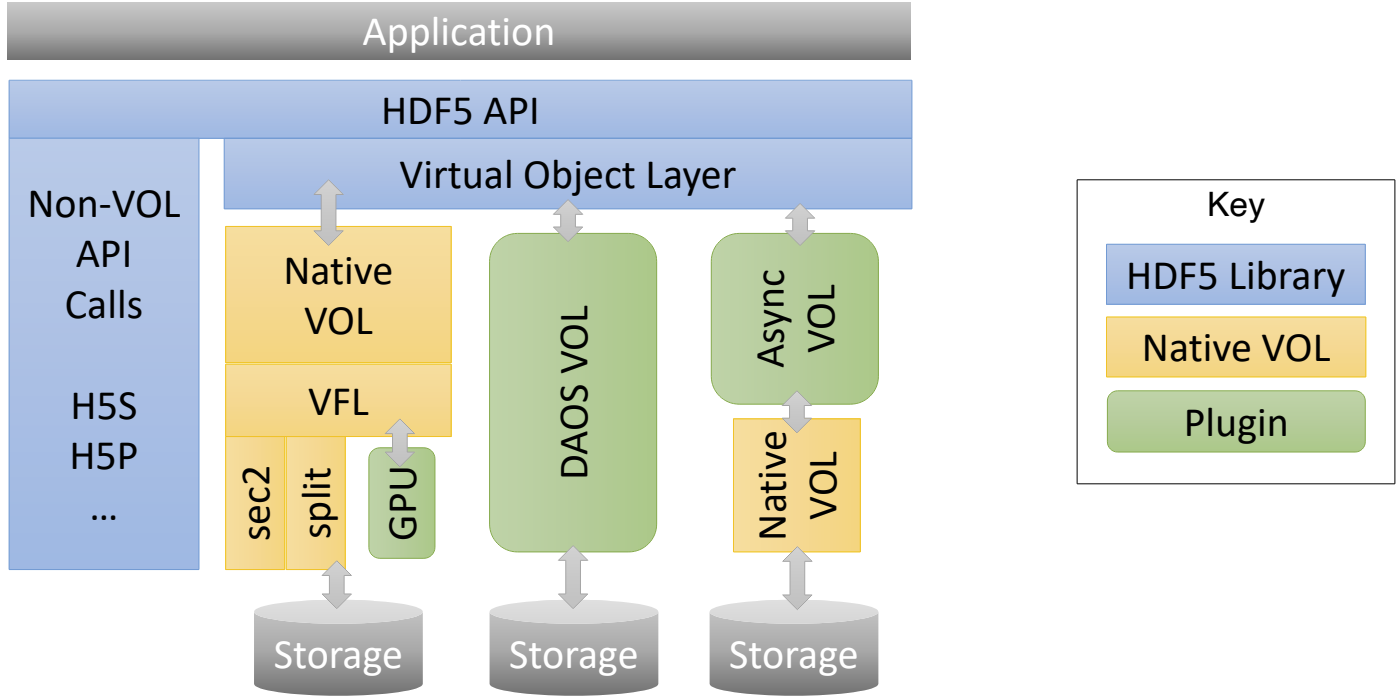
\includegraphics[width=0.7\textwidth]{images/VOL_arch.png}
\caption{The VOL architecture.}
\label{fig:vol-arch}
\end{figure}

The Virtual Object Layer (VOL) is an HDF5 library extension interface for implementing actual mappings of virtual objects to storage and implementing the operations associated with such objects' life cycle (creation, deletion, copying, etc.). Modules implementing such mappings are called VOL \textit{connectors} and are typically packaged as dynamically loadable plugins. In Figure~\ref{fig:vol-arch}, three VOL connector examples are shown: the so-called `Native VOL', the DAOS VOL~\cite{soumagne2021}, and the Async VOL~\cite{tang2020}. Notice that certain VOL connectors are stackable and that the native VOL is \textit{not} implemented as a plugin. The latter is due to the VOL-centric library architecture being relatively new. It was introduced in HDF5 library release 1.12.0 and underwent a significant revision for the HDF5 1.14.0 release. Before introducing the VOL layer, the HDF5 library was more or less identical to the native VOL connector (plus the non-VOL support functions). Perhaps the main takeaway from Figure~\ref{fig:vol-arch} is that what's now considered the HDF5 library is a lot smaller than expected. Today, the HDF5 library consists of an API, the VOL interface, and a non-VOL API management infrastructure. Of course, that bare-bones library doesn't do anything useful, and we need at least one VOL connector that implements an actual mapping of HDF5 virtual objects to storage.

Since, during this tour, we only examine library initialization and finalization, we will not encounter any ``proper" VOL functions. No virtual objects are constructed or mapped to storage, and no operations are performed on them. We will witness the initialization and finalization of the library's non-VOL infrastructure and the native VOL packages. During subsequent tours, we will see the native VOL in action, i.e., mapping HDF5 virtual objects to files formatted according to the HDF5 file format specification~\cite{ffmt} via the native VOL's Virtual File Layer (VFL) extension interface.

Unless stated otherwise and to keep the discussion simple, in this chapter, we include the native VOL connector when we refer to the HDF5 library. As we saw, however, this is not entirely true.

In this section, we describe the life cycle of an HDF5 library instance running in the context of an application process. This includes lazy library initialization, dynamic configuration, and finalization. At the end of this section, the reader should have enough information to answer the following questions:

\begin{itemize}
    \item What does it mean for a library instance to be initialized/finalized?
    \item What triggers a library instance initialization/finalization?
    \item What's the sequencing of library initialization/finalization?
    \item As a library developer, what library changes require careful consideration of/coordination with library initialization/finalization?
\end{itemize}

\paragraph{Prototype.} Consider the HDF5 version of a ``Hello, World!" program shown in Listing~\ref{lst:explicit-init}. The naming \func{H5[open,close]} is perhaps a little misleading (Why not \func{H5[init,finalize]}?), but, for reasons which will become clear later, most users and developers will never call these two functions directly.

\begin{listing}[H]
\caption{Explicit HDF5 library run-time initialization and finalization.}
\label{lst:explicit-init}
\begin{minted}[linenos]{C}
#include "common.h"
int main() {
    H5open();
    printf("Hello, HDF5!\n");
    H5close();
    return 0;
}
\end{minted}
\end{listing}


\paragraph{Goals.} The main goals of library initialization and finalization are:

\begin{itemize}
    \item Setup and tear-down of error handling infrastructure
    \item Module initialization and finalization, including
    \begin{itemize}
        \item (De-)Registration of API entity types (or classes)
        \item Initialization and finalization of global variables
        \item Retrieval of environment variables, e.g., for the discovery of plugin paths
    \end{itemize}
\end{itemize}

\paragraph{Control flow.} A cursory inspection of the call graph of the program shown in Listing~\ref{lst:explicit-init} suggests that \func{H5[open,close]} proceed directly to \func{H5_[init,term]_library}, respectively.

\func{H5_init_library} is responsible for calling the initializers of all non-VOL and native VOL library modules (aka ``packages") in the correct order so that no module is initialized before its prerequisite modules. A table in \func{H5_init_library} establishes the order of initialization. The table, as implemented at the time of this writing, is shown in Listing~\ref{lst:init-table}.

\begin{listing}
\centering
\caption{\texttt{H5\_init\_library()} initialization table.}
\label{lst:init-table}
\begin{minted}[linenos]{C}
struct {
    herr_t (*func)(void);
    const char *descr;
} initializer[] = {
    {H5E_init, "error"}
,   {H5VL_init_phase1, "VOL"}
,   {H5SL_init, "skip lists"}
,   {H5FD_init, "VFD"}
,   {H5_default_vfd_init, "default VFD"}
,   {H5P_init_phase1, "property list"}
,   {H5AC_init, "metadata caching"}
,   {H5L_init, "link"}
,   {H5S_init, "dataspace"}
,   {H5PL_init, "plugins"}
/* Finish initializing interfaces that depend on the interfaces above */
,   {H5P_init_phase2, "property list"}
,   {H5VL_init_phase2, "VOL"}
};
\end{minted}
\end{listing}

Most package initializers (the \texttt{H5*\_init*} routines) register identifier classes or check environment variables. The only notable exception is the \texttt{H5T} package initializer, which initializes identifiers (stored in global variables) for built-in datatypes and several pre-defined datatype transformations. For this tour, where we do not encounter any identifiers, it is sufficient to know that identifiers are ephemeral handles of API type \texttt{hid\_t}, which the library uses to track API entities. For efficiency and error checking, the identifier space is ``partitioned'' into identifiers of different types, and developers can create (register) custom identifier types to track their entities.

As the table shows, a few modules (\texttt{H5P,H5VL}) require phased initialization. \texttt{H5\_default\_vfd\_init()}, in connection with \texttt{H5P\_init\_phase2()},  registers and initializes the POSIX VFD as the default file driver. Finally, \texttt{H5VL\_init\_phase2()} initializes the remaining modules according to a similar table shown in Listing~\ref{lst:vol2-init-table}.

\begin{listing}
\centering
\caption{\texttt{H5VL\_init\_phase2()} initialization table.}
\label{lst:vol2-init-table}
\begin{minted}[linenos]{C}
struct {
    herr_t (*func)(void);
    const char *descr;
} initializer[] = {
    {H5T_init, "datatype"}
,   {H5O_init, "object header"}
,   {H5D_init, "dataset"}
,   {H5F_init, "file"}
,   {H5G_init, "group"}
,   {H5A_init, "attribute"}
,   {H5M_init, "map"}
,   {H5CX_init, "context"}
,   {H5ES_init, "event set"}
,   {H5Z_init, "transform"}
,   {H5R_init, "reference"}
};
\end{minted}
\end{listing}

\texttt{H5VL\_init\_phase2()} concludes the HDF5 library initialization.

Only \texttt{H5[A,D,F,G,L,M,T]} API functions will pass through the VOL layer; all other packages support non-VOL API calls or library internal infrastructure.

\noindent\fbox{\parbox{\linewidth}{At this point, the library would be considered initialized with its default configuration (native VOL + POSIX VFD), and the application can proceed to create and manipulate HDF5 virtual objects that are mapped to HDF5 files in a POSIX-compliant file system. For other mappings, different VOL connectors or VFD plugins would be required.}}

The library has a default behavior to shut down when the application exits by registering an \texttt{atexit(3)} handler, \func{H5_term_library}. This will invoke modules' \func{H5*_[top]_term_package} functions. The shutdown table is too extensive to be repeated here. It is also heavily commented on and should be consulted for more in-depth information. Akin to the phased initialization for certain modules, the finalization of a few modules is split into ``top" and ``bottom" portions. Note that some entries in the shutdown table are marked as ``barriers," and if a new module should only be shutdown \textit{strictly after} the preceding modules, then it should be marked as a barrier. This is achieved by setting the \texttt{wait} parameter of the \texttt{TERMINATOR} macro for the corresponding module to \texttt{true}.

\paragraph{Data flow.} The library's initialization and finalization state are tracked in two global variables, namely \texttt{H5\_INIT\_GLOBAL} and \texttt{H5\_TERM\_GLOBAL}. These variables are specifically set by two library functions \texttt{H5\_init\_library()} and \texttt{H5\_term\_library()}, respectively. The initialization and finalization of library modules typically involve registering and unregistering module-specific identifier types (for example, \texttt{H5I\_DATASPACE\_CLS} and \texttt{H5I\_SPACE\_SEL\_ITER\_CLS} for \texttt{H5S}) and the initialization/finalization of module-specific global variables. Perhaps the most elaborate example is \texttt{H5T}, which requires the initialization/finalization of built-in datatypes such as \texttt{H5T\_IEEE\_F64BE\_g} and conversion functions such as \texttt{H5T\_\_conv\_double\_ldouble()} in the global variable \texttt{H5T\_g}. Otherwise, there is very little data flow activity during library initialization/finalization.

\begin{listing}
\centering
\caption{Implicit HDF5 library initialization.}
\label{lst:implicit-init}
\begin{minted}[linenos]{C}
#include "common.h"
int main() {
  unsigned int majnum, minnum, relnum;
  H5get_libversion(&majnum, &minnum, &relnum);
  printf("Hello, HDF5 %u.%u.%u!\n", majnum, minnum, relnum);
  return 0;
}
\end{minted}
\end{listing}

\paragraph{Variants.} In Listing~\ref{lst:implicit-init}, a variant of the ``Hello, World!" example is shown. The notable difference is the new function \func{H5get_libversion}, while the previous version had calls to \func{H5open} and \func{H5close}, which have been removed in the new version. It turns out that the HDF5 library initializes itself as needed whenever an application either enters the library through an API function call such as \texttt{H5get\_libversion()}, or when an application evaluates an HDF5 symbol that represents a macro such as \texttt{H5F\_ACC\_RDONLY} or \texttt{H5F\_ACC\_RDWR}, a property-list class identifier such as \texttt{H5P\_FILE\_ACCESS}, a VFD identifier such as \texttt{H5FD\_FAMILY} or \texttt{H5FD\_SEC2}, or a type identifier
such as \texttt{H5T\_NATIVE\_INT64}.

The library provides a couple of macros that initialize the library as necessary. Library initialization is checked as a side-effect of the \texttt{FUNC\_ENTER\_API*} macros used at the top of most API functions. HDF5 library symbols other than functions are provided through \texttt{\#define}s that use the \texttt{H5OPEN} macro to introduce a library-initialization call (\texttt{H5open()}) at each site where a non-function symbol is used.

Two noteworthy variants of HDF5 library initialization and finalization will be discussed in later tours. One is the case of MPI-parallel HDF5
%(see section~\ref{sec:MPI-state-n-sync})
, where multiple library instances simultaneously operate on one or more files with different sharing patterns. The other one is the use case of a library built with thread-safety enabled  (see section~\ref{sec:H5TS-impl}). In both cases, the changes to HDF5 library initialization and finalization are ``around the edges" and deal with MPI initialization, finalization, and API lock management, respectively.



\paragraph{Developer considerations.} When a developer exports a new symbol as part of the HDF5 library, they should ensure that an application cannot enter the library in an uninitialized state through a new API function or read an uninitialized value from a non-function HDF5 symbol.

If a developer adds a module to the library that must be initialized with the rest of the library, then they should insert its initializer into the right place in the table.

If a developer adds a module that needs to release resources during library shutdown, they should add a call to the shutdown table at the right place.

\paragraph{Source code recommended for study.}

\begin{itemize}
    \item \texttt{H5\_[init,term]\_library()} in \texttt{H5.c}
    \item \texttt{H5E\_[init,term]\_package()} in \texttt{H5E.c}
    \item \texttt{H5T\_init(), H5T\_top\_term\_package()} in \texttt{H5T.c}
    \item \texttt{H5VL\_init\_phase2()} in \texttt{H5VLint.c}
\end{itemize}

\subsection{Summary}

\begin{figure}[h]
\centering
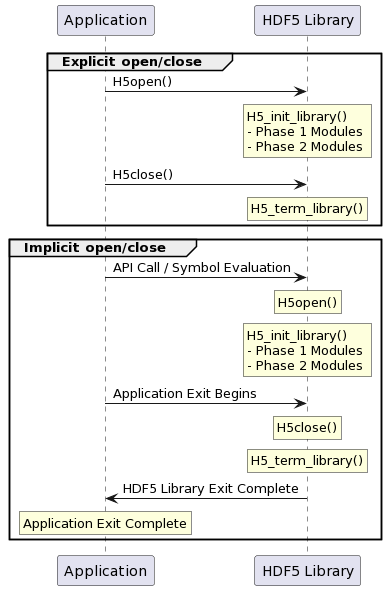
\includegraphics[width=0.5\textwidth]{images/tour_1_uml.png}
\label{fig:tour-1-uml}
\caption{Library initialization/termination sequence diagram.}
\end{figure}

Given the substantial library infrastructure we have seen during this tour, it is too easy to ``miss the architecture for the code". The key takeaway from this tour is that, as suggested in Figure ~\ref{fig:vol-arch}, the HDF5 library consists of
\begin{enumerate}
    \item A (C-) API
    \item An extension interface (VOL) to implement mappings between HDF5 virtual objects and storage representations
    \item A supporting infrastructure (non-VOL) for API handle management, API properties, etc.
    \item A default mapping (native VOL) between HDF5 virtual objects and the content of files formatted according to the HDF5 file format specification~\cite{ffmt}.
\end{enumerate}

Library initialization and finalization are usually triggered by API entry and an \texttt{atexit(3)} handler. The HDF5 library source code is organized modularly, and initialization and finalization proceed through modules in a defined order, respecting inter-module dependence. Developers must guard against uncontrolled API entrance, violations of module interdependence during library initialization and shutdown, and failures to release unused resources.